% !TEX root = ../gw.tex

\section{Introduction}

%\gabriel{I found that one thing that is missing, in both abstract/introduction and also a bit in the numerics (put aside partial matching) is that we actually deal with "measured metric spaces". It is a distinctive features from classical matching methods and allows to take into account e.g. some kind of uncertainty in the inputs.}

A basic component of the geometry processing toolbox is a tool for \emph{mapping} or \emph{correspondence}, the problem of finding which points on a target domain correspond to points on a source.  Many variations of this problem have been considered in the graphics literature, e.g.\ with some sparse correspondences provided by the user.  Regardless, the basic task of geometric correspondence facilitates the transfer of properties and edits from one shape to another.

The primary factor that distinguishes correspondence algorithms is the choice of objective functions. Different choices of objective functions express contrasting notions of which correspondences are ``desirable.''  Classical theorems from differential geometry and most modern algorithms consider \emph{local} distortion, producing maps that take tangent planes to tangent planes with as little stretch as possible; slightly larger neighborhoods might be taken into account by e.g.\ aligning heat kernels.  These approaches are justified by classical differential geometry when the matched domains satisfy conditions like near-isometry or near-conformality, but when these conditions are violated these algorithms suffer from having to patch together local elastic terms into a single global map. 

%\suv{Note on style: If possible, avoid using too many gerunds, i.e., ``...ing'' constructions, in favor of directly using verbs; makes the text more readable.}%duly noted!  writing in this paper in part is optimized a bit for space rather than clarity, although that's no excuse for poor exposition :-)

In this paper, we propose a new correspondence algorithm that minimizes distortion of long- and short-range distances alike.  We study an entropically-regularized version of the \emph{Gromov-Wasserstein} (GW) mapping objective function from~\cite{memoli-2011} measuring the distortion of geodesic distances.  The optimizer is a probabilistic matching expressed as a ``fuzzy'' correspondence matrix in the style of~\cite{kim-2012,solomon-2012}; %\gabriel{yes, but at the end of the day, what makes the matrix really fuzzy (at least in the setting where the 2 spaces have the same number of points) is rather the introduction of the entropy. Don't you think ? }
we control sharpness of the correspondence via the weight of an entropic regularizer.   

 Although~\cite{memoli-2011} and subsequent work identified the possibility of using GW distances for geometric correspondence, computational challenges hampered their practical application.  To overcome these challenges, we build upon recent methods for regularized optimal transportation introduced in~\cite{benamou-2015,solomon-2015}.  While optimal transportation is a fundamentally different optimization problem from regularized GW computation (linear versus quadratic matching), the core of our method relies upon solving a sequence of regularized optimal transport problems. %\gabriel{I am not sure the average reader will get the idea. Shouldn't you be more direct and say "resolution of a sequence of simpler regularized optimal transports (i.e. regularized linear programs) comprises ..."}

Our remarkably compact algorithm (see Algorithm~\ref{alg:gw}) exhibits global convergence, i.e., it \emph{provably} reaches a local minimum of the regularized GW objective function regardless of the initial guess.  Our algorithm can be applied to any domain expressible as a metric measure space (see \S\ref{sec:related_work}).  Concretely, only distance matrices are required as input, and hence the method can be applied to many classes of domains including meshes, point clouds, graphs, and even more abstract  structures. 

A major advantage of our framework is its extensibility.  In addition to the conventional correspondence problem, we apply our method to organizing shape collections and show how to find correspondences given user guidance or incomplete pairwise distances.  We also provide algorithms to extract multiple maps in the presence of symmetry and to compute consistent maps within a collection.% via a connection to nonnegative matrix factorization.

%\suv{Is it typical to write this as a para, or can we write out an itemize to make it stand out / be easy for the reviewer?}% I've seen both.  Will change to bullets

\begin{figure}[t]\centering
$
\underbrace{
\includegraphics[height=1in]{figures/icon/icon_source.pdf}
}_{\textrm{Source}}
%\mapsto
\underbrace{
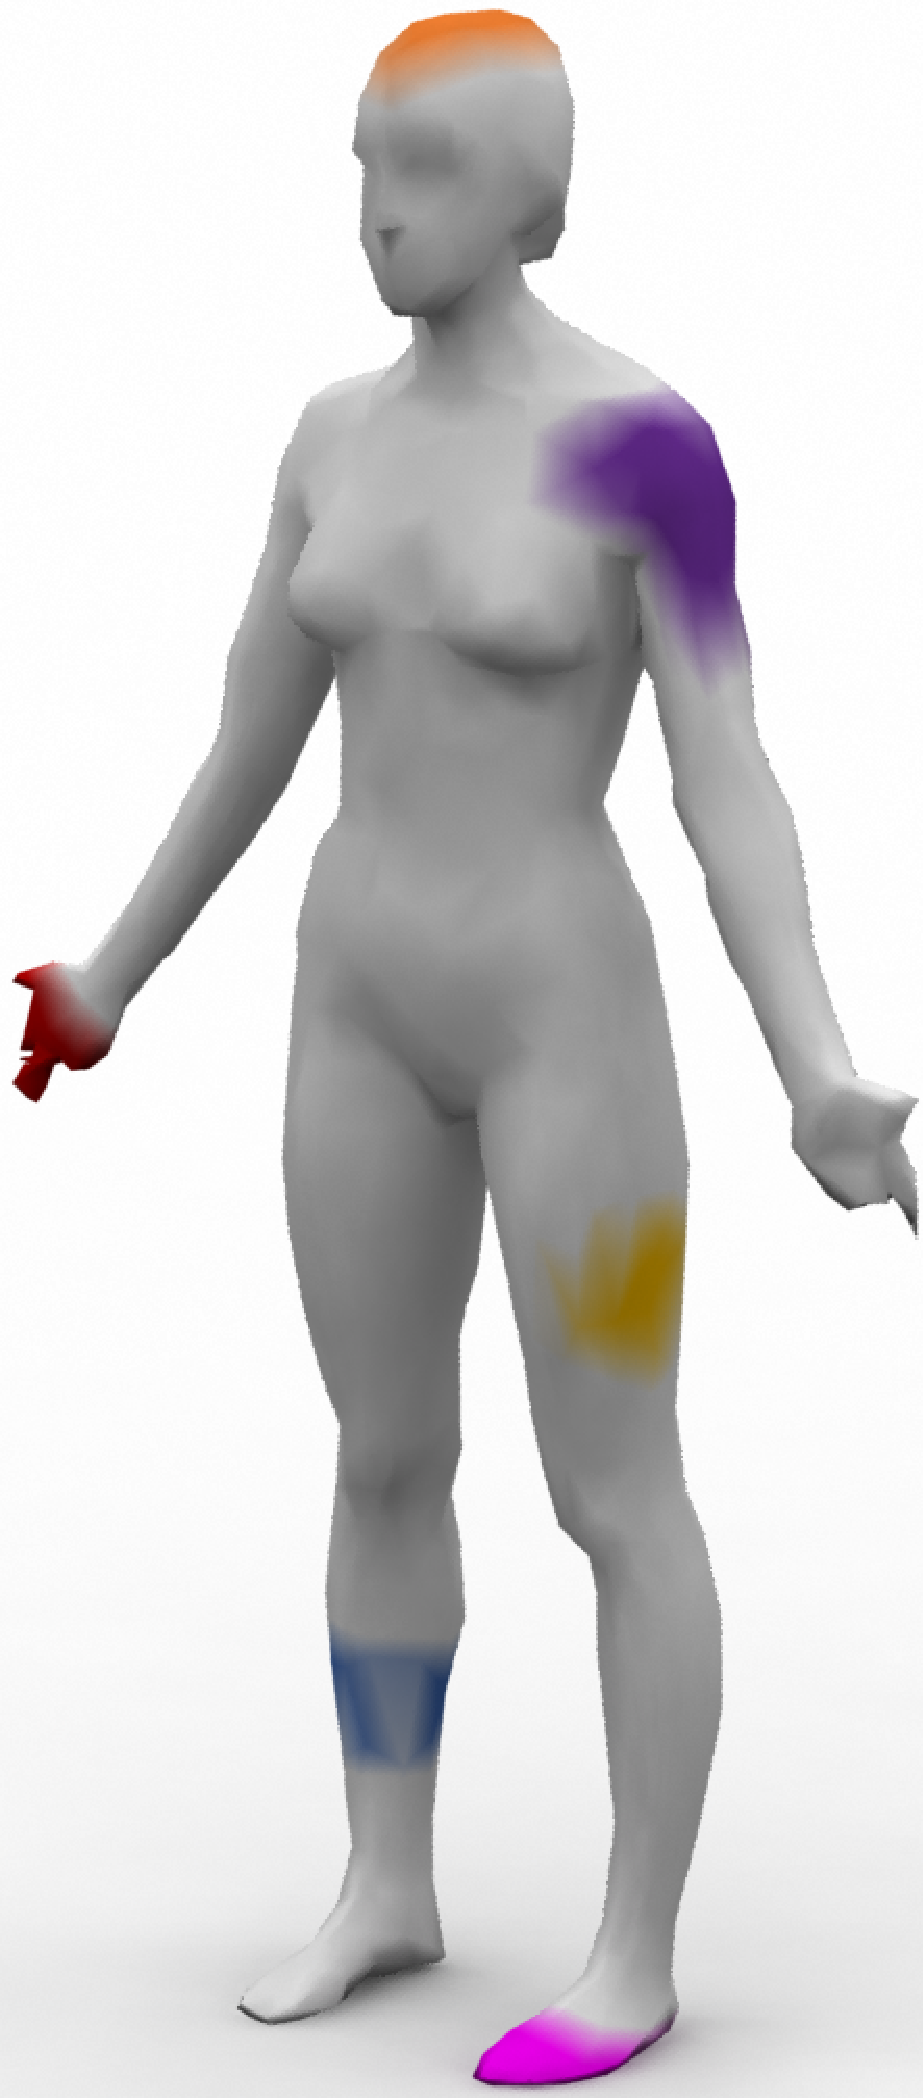
\includegraphics[height=1in]{figures/surface_maps/target_skirt2.pdf}
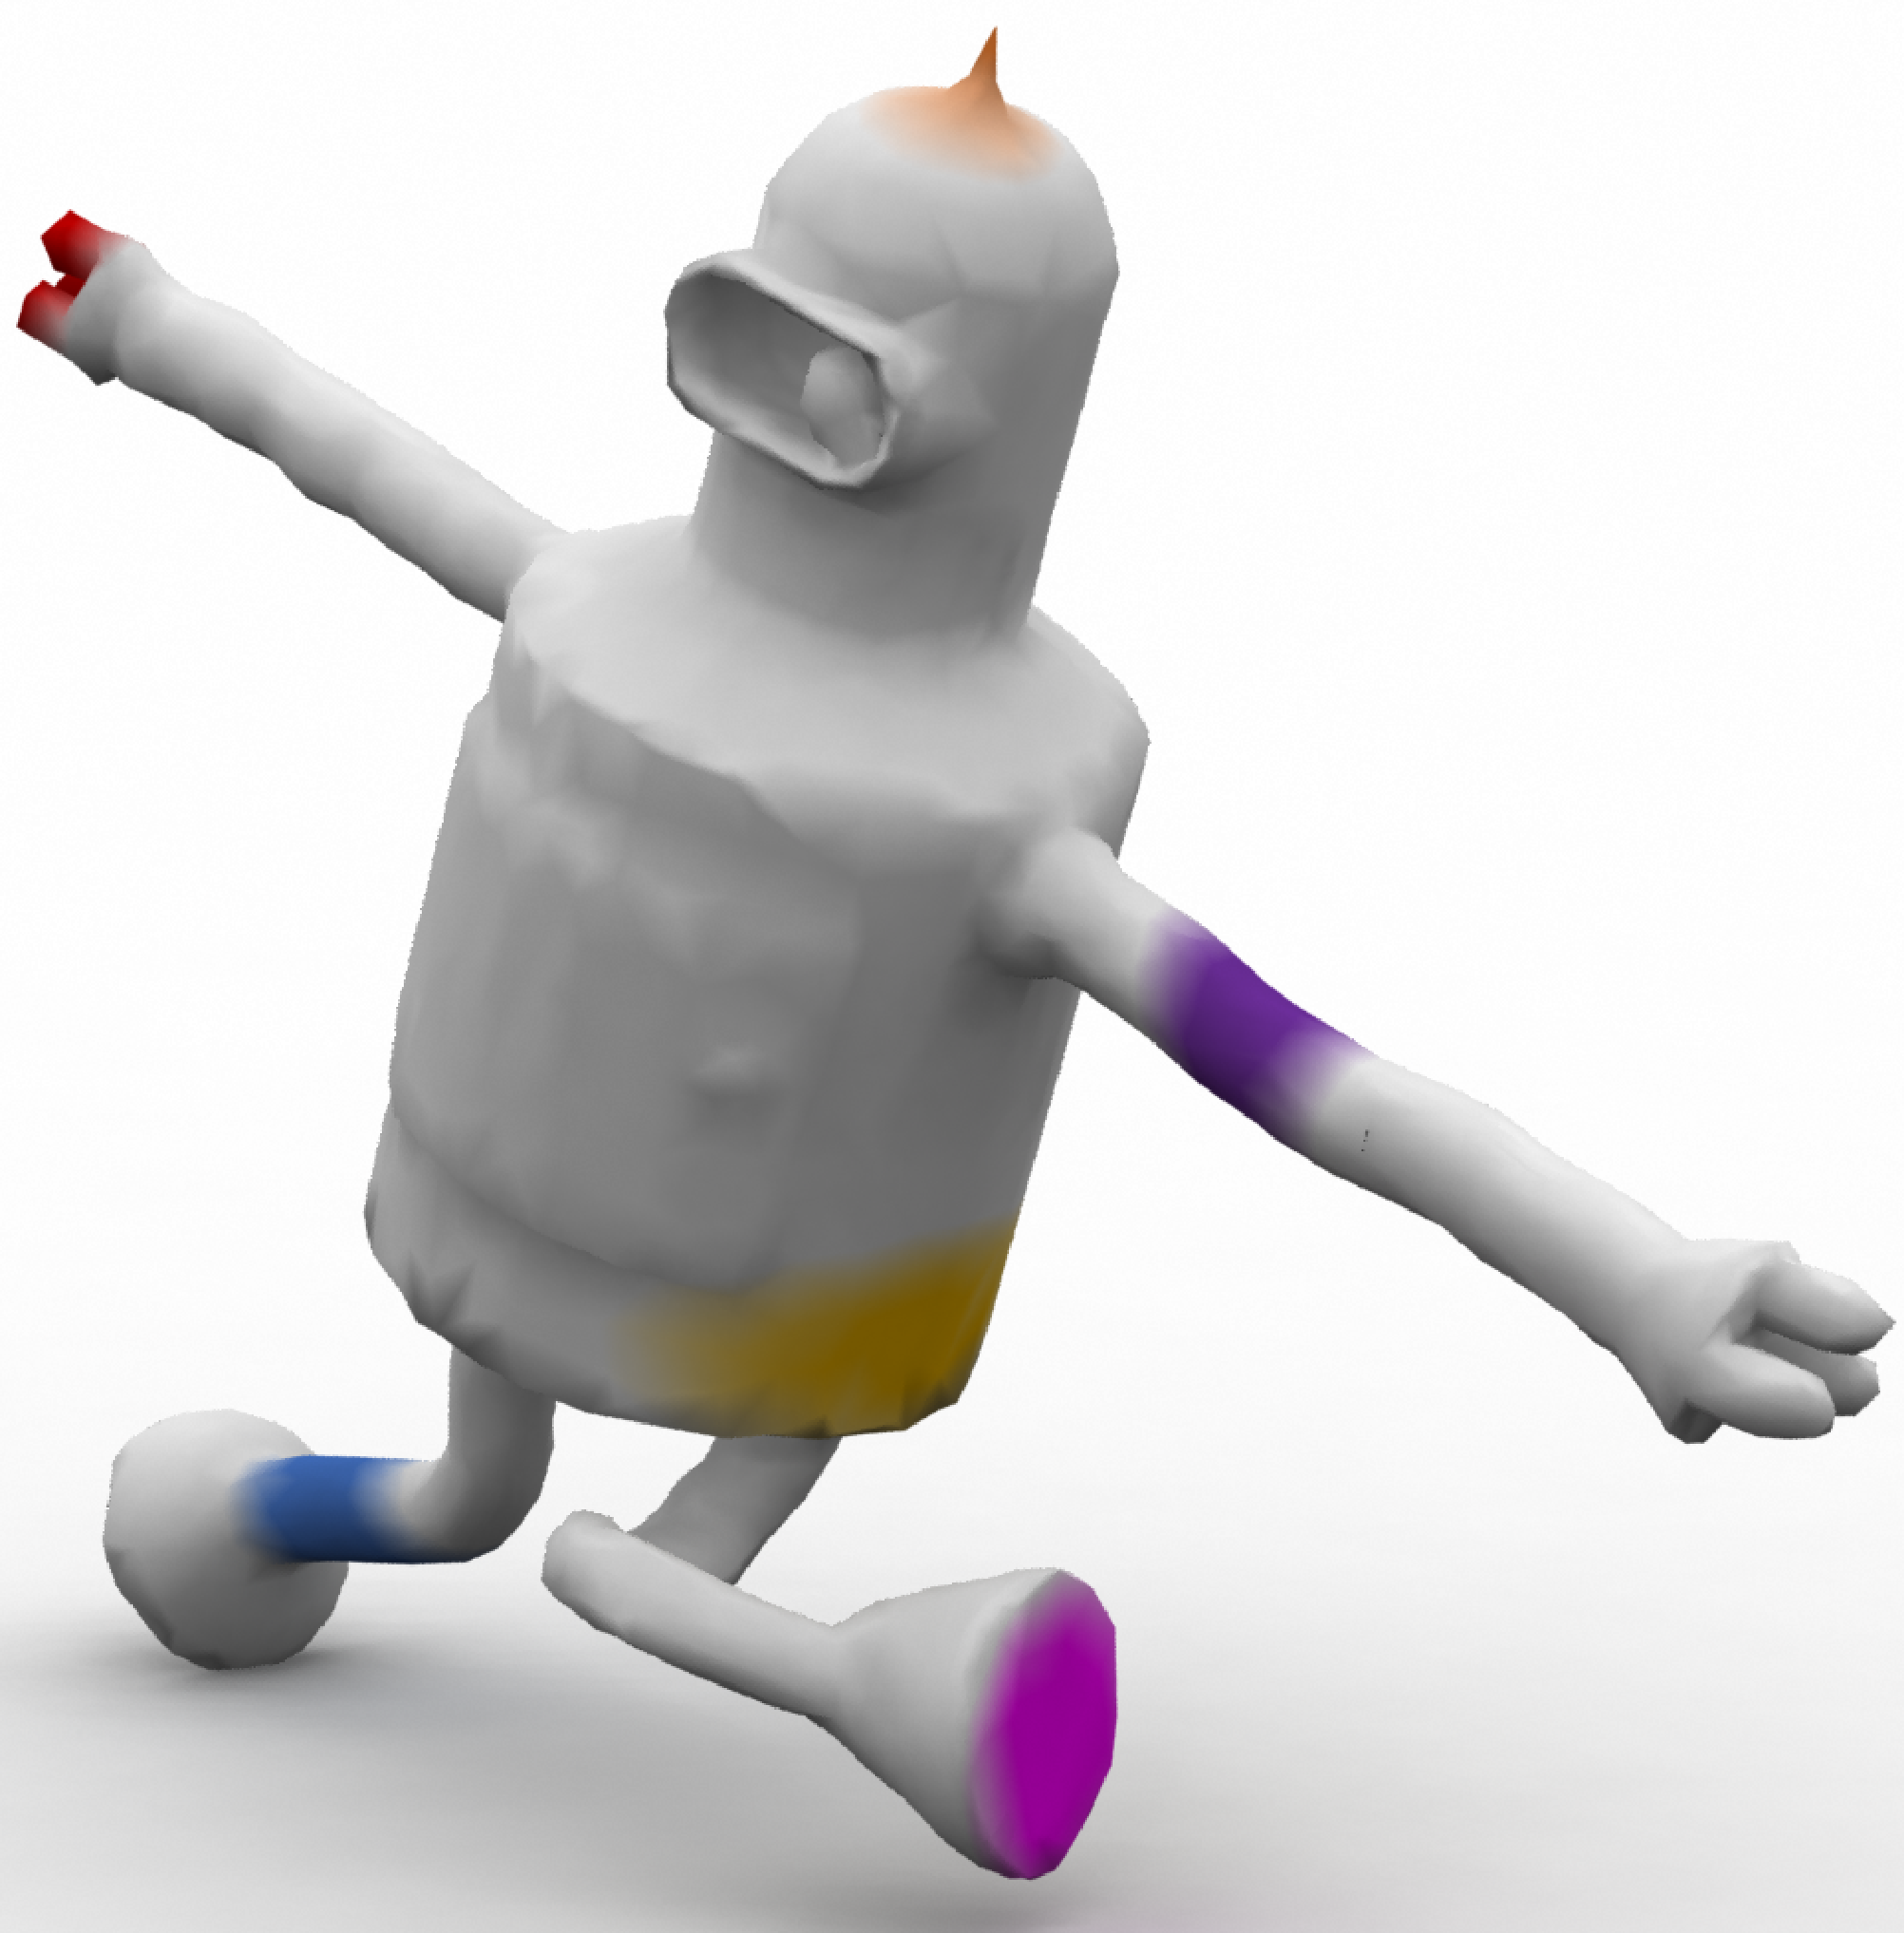
\includegraphics[height=1in]{figures/surface_maps/target_skirt.pdf}
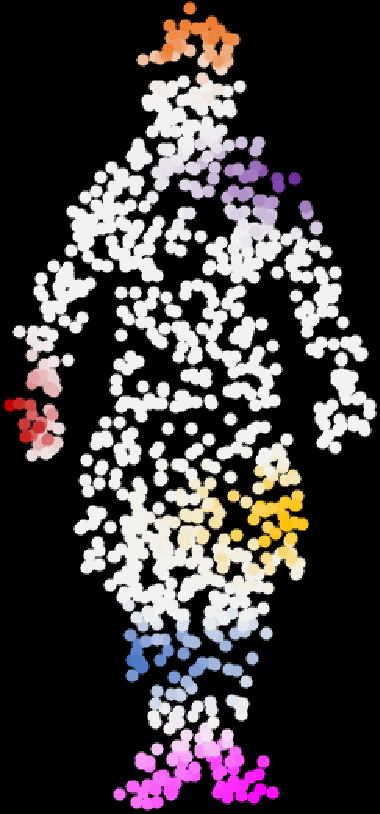
\includegraphics[height=1in]{figures/cloud/cloud2.pdf}
\includegraphics[height=1in]{figures/icon/icon_target.pdf}
\includegraphics[height=1in]{figures/icon/icon_target2.pdf}
}_{\textrm{Targets}}
$
\vspace{-.1in}
\caption{Entropic GW can find correspondences between a source surface (left) and a surface with similar structure, a surface with shared semantic structure, a noisy 3D point cloud, an icon, and a hand drawing. Each fuzzy map was computed using the same code.\vspace{-.2in}}\label{fig:shape_to_icon}
\end{figure}

\paragraph*{Contributions.} We present a fuzzy mapping algorithm minimizing the Gromov-Wasserstein (GW) objective with entropic regularization. In summary, our key contributions are the following: %Specifically, we introduce the following:
\begin{itemize}[topsep=0pt,itemsep=-1ex,partopsep=1ex,parsep=1ex]
\item discretization of an entropically-regularized GW objective suitable for domains in graphics and geometry processing;
\item a simple-to-implement algorithm for minimizing this objective that relies only upon scalable low-level linear algebra;
\item a convergence proof for the iterative optimization algorithm;
\item comprehensive experiments establishing reliability, efficiency, and versatility of the regularized GW algorithm; and
\item proof-of-concept extensions of regularized GW correspondence to a large variety of problems, demonstrating its versatility within the geometry processing and graphics toolboxes.%extensions of regularized GW correspondence to shape exploration, supervised matching, uncertain distance matrices, symmetry detection, and joint domain analysis.
\end{itemize}

%It is simple to implement, applicable to many types of domains, and relies only upon scalable low-level linear algebra.  We provide careful consideration of convergence properties. In addition to evaluating our technique applied to a variety of matching tasks, we show how it can be extended and modified to handle variations of the basic problem, including matching from incomplete distance data and joint domain mapping.
%\justin{to add:  faster than existing fuzzy maps tools}

%\suv{Should related work be Section 1.1 or an entire separate section as of now?}% Usually I've seen SIGGRAPH papers where it's section 2.

% note somewhere --  yaron's sdp for controlling singular values doesn't show it reaches a local min




%Several considerations determine the effectiveness of a technique for correspondence.  From a theoretical standpoint, correspondence algorithms can be judged based on their induced distortion on different classes of shapes, resilience to ambiguity or ill-posedness in the matching problem, and applicability to different geometric representations.  Algorithmic considerations include efficiency or control over the trade-off between accuracy and runtime.  Finally, ease of use, ease of implementation, and the option to provide supervision can make the technique more controllable by an end user.
%
%Countless optimization-based mapping algorithms pose the problem as the minimization of a quadratic objective subject to assorted constraints.  Intuitively, the quadratic term usually measures continuity of the computed map, preferring maps that take nearby points on the source surface to nearby points on the target.  Discrete versions seeking point-to-point maps likely are algorithmically intractable---even within a constant approximation factor~\cite{sahni-1976}---and after relaxing integer constraints the problem remains similarly intractable~\cite{sahni-1974}.
%
%For this reason, quadratic correspondence techniques generally either work with a convexification of the original problem or lack convergence guarantees or global optimality.  The former approach has gained popularity due to the possibility of proving guarantees on the quality of the output and/or certificates of optimality, at the expense of having to solve large-scale convex problems that severely limit the number of matched points~\cite{solomon-2013,kezurer-2015}.  Furthermore, these relaxations can have large convex hulls of optimal solutions when the mapping problem admits even a discrete symmetry.  Contrastingly, simpler heuristic approaches to mapping might be considered approximations to the original nonconvex problem with few guarantees.
%
%In this paper, we bridge between these extremes with a mapping algorithm for the original nonconvex mapping problem that is straightforward to implement using simple and relatively efficient iterations.  Despite its simplicity, the algorithm is \emph{provably} convergent to a critical point of the objective regardless of the initial guess, and the convergence rate appears to be sufficient for practical use.
%
%In particular, we propose algorithms for optimizing a regularized version of the \emph{Gromov-Wasserstein} objective seeking maps between surfaces that preserve pairwise geodesic distances; in the absence of isometry, this objective promotes minimal distortion of the geodesic structure of the domain.  While this approach to matching was proposed in~\cite{memoli-2011}, the underlying numerical problem presented significant challenges that led to the proposal of aggressive spectral approximations that are far more sensitive to deviation from isometry~\cite{memoli-2009}.
%
%Furthermore, we extend our technique to computation of consistent maps within a collection.  We propose a completely unsupervised pipeline incorporating consistency into the mapping pipeline rather than enforcing it \emph{a posteriori}.  Our approach is made possible via a connection to nonnegative matrix factorization (NMF) techniques appearing in the machine learning literature.
%
%We demonstrate our computational techniques on a variety of computational techniques, including not only shape matching but also \justin{TBD.}
%
%\paragraph*{Contributions.} \justin{Write me last.}


%%% Local Variables:
%%% mode: latex
%%% TeX-master: "../gw"
%%% End:
